\documentclass[12pt]{article}

\input ../exam-setup
\newcommand{\version}{}
\newcommand{\factoid}{}
\newcommand{\aquestion}{}
\newcommand{\bquestion}{}
\newcommand{\cquestion}{}
\newcommand{\hinttext}{}

\newcommand{\ExamName}{Quiz \#3\version}
% \newcommand{\CourseName}{Math 34A}

\begin{document}
%%
%%
%% Version 1:
\renewcommand{\version}{a}
\renewcommand{\factoid}{10^{0.47}\approx 2.95}
\renewcommand{\aquestion}{\log(295)}
\renewcommand{\bquestion}{\log(0.0295)}
\renewcommand{\cquestion}{10^{-0.53}}
\renewcommand{\hinttext}{-0.53 = -1 + 0.47}

\setcounter{problemnumber}{0}
\begin{minipage}{0.25\linewidth}
  \CourseName\ \Quarter \\
  \ExamName \\[1em]
  \textbf{No calculators}\\[2em]
\end{minipage}
\hfill
\begin{minipage}[t]{0.4\linewidth}
  
\begin{tikzpicture}[x=26mm,y=16mm]
    \draw[thick,black] (0,0) rectangle (3,1);
    \node[\faintcolor,right] at (0,0.2) {\large\textsf{PRINT NAME}};
  \end{tikzpicture}
\end{minipage}
\hfill
\begin{minipage}{0.25\linewidth}
  \vspace*{-3.25em}
  \ \hfill
  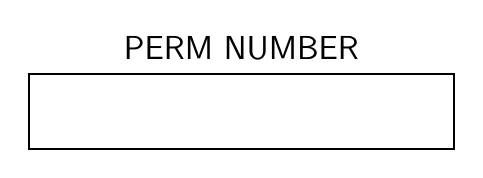
\begin{tikzpicture}[x=36mm,y=16mm]
    \node[\faintcolor] at (0.75,0.8) {\large\textsf{PERM NUMBER}};
    \draw[thick,black] (0,0) rectangle (1.5,0.6);
  \end{tikzpicture}
\end{minipage}
% \medskip
\vspace*{-0.25in}

Put your answer in the 
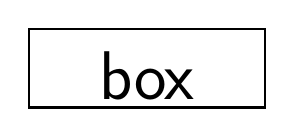
\begin{tikzpicture}[x=10mm,y=10mm,baseline=3mm] 
  \draw[thick,black] (0,0) rectangle (3,1);
  \node[\faintcolor] at (1.5,0.4) {\Huge\textsf{box}};
\end{tikzpicture}
provided.
\hfill
\begin{minipage}{0.5\linewidth}
  \textbf{TA:}\ 
  \parbox[t]{0.7in}{%
    \checkbox\ \TAOne \\
    \checkbox\ \TATwo 
  }
  \parbox[t]{0.7in}{%
    \checkbox\ \TAThree\\
    \ \ \ 
  }
  % \ 
  % \parbox[t]{4in}{%
  % \textbf{Section Time:}
  \hfill%\hspace*{0.25in}
  % \ 
  % \parbox[t]{4in}{%
  % \textbf{Section Time:}
  \textbf{Time:}
  \parbox[t]{0.55in}{%
    \checkbox\ 8am \\
    \checkbox\ 5pm
  }
  \quad
  \parbox[t]{0.55in}{%
    \checkbox\ 6pm \\
    \checkbox\ 7pm 
  }
  % }
\end{minipage}
\noindent\hspace*{-2em}\rule{\textwidth+4em}{1pt}%

\begin{enumerate}
  \Problem %\Points{3} %
  \parbox[t]{5.75in}{We are told that $\factoid$.  Find (a) $\aquestion$,
    (b) $\bquestion$, and (c) $\cquestion$. \\[0.5em]
    \textbf{Hint:}\ $\hinttext$}


  \ 
  \hfill
  (a) $\aquestion \approx$
  
\begin{tikzpicture}[x=20mm,y=12mm,baseline={6mm}]
    \draw[thick,black] (0,-0.2) rectangle (2,1.2);
    % \node at (1.8,0.5) {\large\%};
  \end{tikzpicture}
  \vspace*{2in}
  
  \ 
  \hfill
  (b) $\bquestion \approx$
  
\begin{tikzpicture}[x=20mm,y=12mm,baseline={6mm}]
    \draw[thick,black] (0,-0.2) rectangle (2,1.2);
    % \node at (1.8,0.5) {\large\%};
  \end{tikzpicture}
  \vspace*{2in}
  
  \ 
  \hfill
  (c) $\cquestion \approx$
  
\begin{tikzpicture}[x=20mm,y=12mm,baseline={6mm}]
    \draw[thick,black] (0,-0.2) rectangle (2,1.2);
    % \node at (1.8,0.5) {\large\%};
  \end{tikzpicture}
\end{enumerate}
\newpage
%%
%%
%% Version 2:
\renewcommand{\version}{c}
\renewcommand{\factoid}{10^{0.66} \approx 4.57}
\renewcommand{\aquestion}{\log(457)}
\renewcommand{\bquestion}{\log(0.0457)}
\renewcommand{\cquestion}{10^{-0.34}}
\renewcommand{\hinttext}{-0.34 = -1 + 0.66}

\setcounter{problemnumber}{0}
\begin{minipage}{0.25\linewidth}
  \CourseName\ \Quarter \\
  \ExamName \\[1em]
  \textbf{No calculators}\\[2em]
\end{minipage}
\hfill
\begin{minipage}[t]{0.4\linewidth}
  
\begin{tikzpicture}[x=26mm,y=16mm]
    \draw[thick,black] (0,0) rectangle (3,1);
    \node[\faintcolor,right] at (0,0.2) {\large\textsf{PRINT NAME}};
  \end{tikzpicture}
\end{minipage}
\hfill
\begin{minipage}{0.25\linewidth}
  \vspace*{-3.25em}
  \ \hfill
  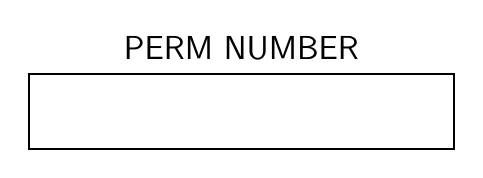
\begin{tikzpicture}[x=36mm,y=16mm]
    \node[\faintcolor] at (0.75,0.8) {\large\textsf{PERM NUMBER}};
    \draw[thick,black] (0,0) rectangle (1.5,0.6);
  \end{tikzpicture}
\end{minipage}
% \medskip
\vspace*{-0.25in}

Put your answer in the 
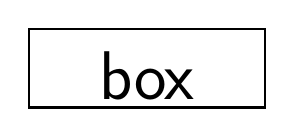
\begin{tikzpicture}[x=10mm,y=10mm,baseline=3mm] 
  \draw[thick,black] (0,0) rectangle (3,1);
  \node[\faintcolor] at (1.5,0.4) {\Huge\textsf{box}};
\end{tikzpicture}
provided.
\hfill
\begin{minipage}{0.5\linewidth}
  \textbf{TA:}\ 
  \parbox[t]{0.7in}{%
    \checkbox\ \TAOne \\
    \checkbox\ \TATwo 
  }
  \parbox[t]{0.7in}{%
    \checkbox\ \TAThree\\
    \ \ \ 
  }
  % \ 
  % \parbox[t]{4in}{%
  % \textbf{Section Time:}
  \hfill%\hspace*{0.25in}
  % \ 
  % \parbox[t]{4in}{%
  % \textbf{Section Time:}
  \textbf{Time:}
  \parbox[t]{0.55in}{%
    \checkbox\ 8am \\
    \checkbox\ 5pm
  }
  \quad
  \parbox[t]{0.55in}{%
    \checkbox\ 6pm \\
    \checkbox\ 7pm 
  }
  % }
\end{minipage}
\noindent\hspace*{-2em}\rule{\textwidth+4em}{1pt}%

\begin{enumerate}
  \Problem %\Points{3} %
  \parbox[t]{5.75in}{We are told that $\factoid$.  Find (a) $\aquestion$,
    (b) $\bquestion$, and (c) $\cquestion$. \\[0.5em]
    \textbf{Hint:}\ $\hinttext$}


  \ 
  \hfill
  (a) $\aquestion \approx$
  
\begin{tikzpicture}[x=20mm,y=12mm,baseline={6mm}]
    \draw[thick,black] (0,-0.2) rectangle (2,1.2);
    % \node at (1.8,0.5) {\large\%};
  \end{tikzpicture}
  \vspace*{2in}
  
  \ 
  \hfill
  (b) $\bquestion \approx$
  
\begin{tikzpicture}[x=20mm,y=12mm,baseline={6mm}]
    \draw[thick,black] (0,-0.2) rectangle (2,1.2);
    % \node at (1.8,0.5) {\large\%};
  \end{tikzpicture}
  \vspace*{2in}
  
  \ 
  \hfill
  (c) $\cquestion \approx$
  
\begin{tikzpicture}[x=20mm,y=12mm,baseline={6mm}]
    \draw[thick,black] (0,-0.2) rectangle (2,1.2);
    % \node at (1.8,0.5) {\large\%};
  \end{tikzpicture}
\end{enumerate}

\end{document}
